\begin{figure}[htbp]
	\centering
  %\null\hfill
  \subfloat[SCT Bayesian linear regressor.]{
	  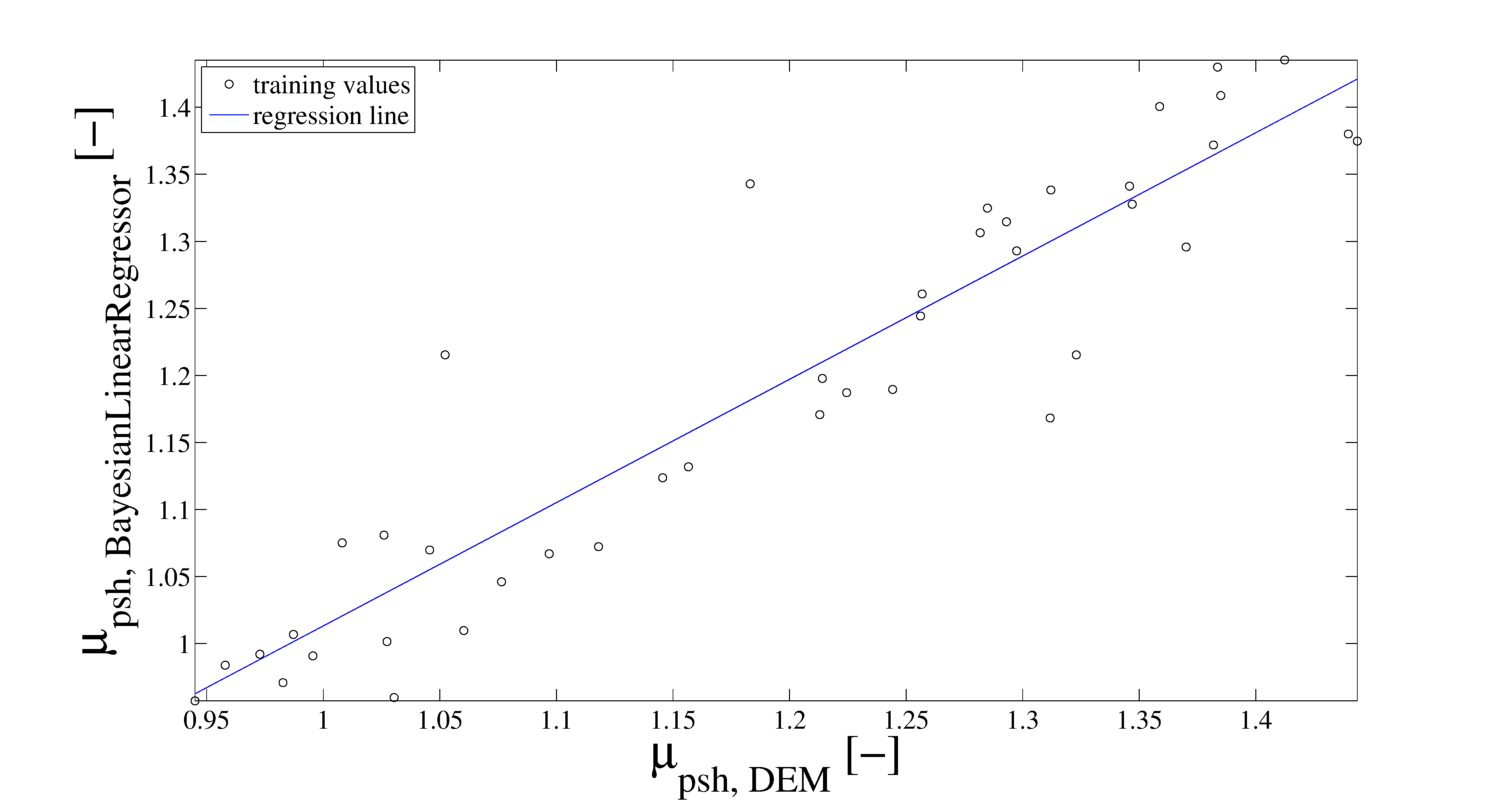
\includegraphics[width=.75\columnwidth]{images/137SCTBayesianLinearRegressor}
	  \label{fig:137SCTBayesianLinearRegressor}
  }
  \\
    \subfloat[SCT Gaussian non linear regressor.]{
	  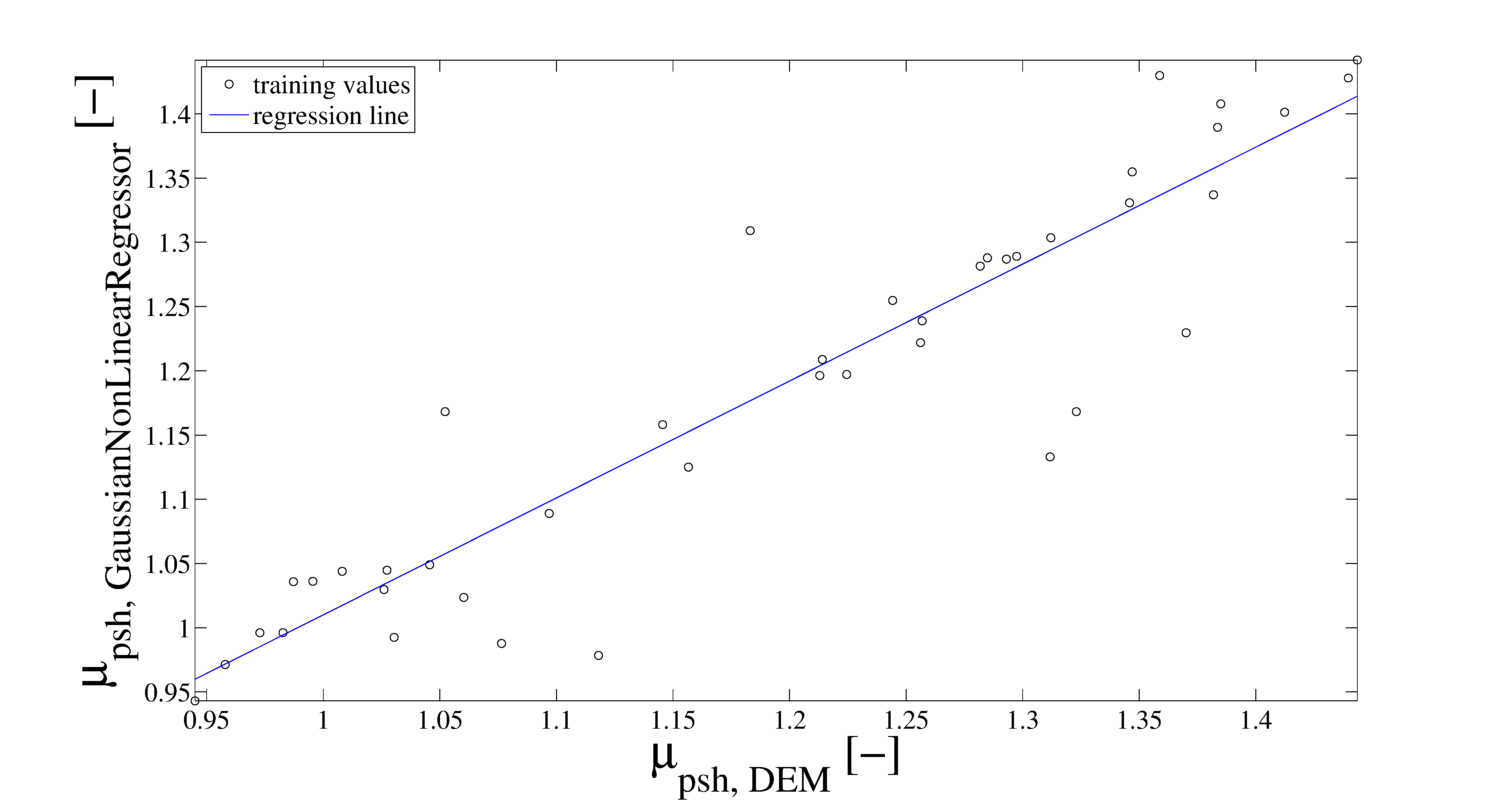
\includegraphics[width=.75\columnwidth]{images/138SCTGaussianNonLinearRegressor}
	  \label{fig:138SCTGaussianNonLinearRegressor}
  }
  \\
 % \hfill
  \subfloat[SCT ANN non linear regression.]{
	  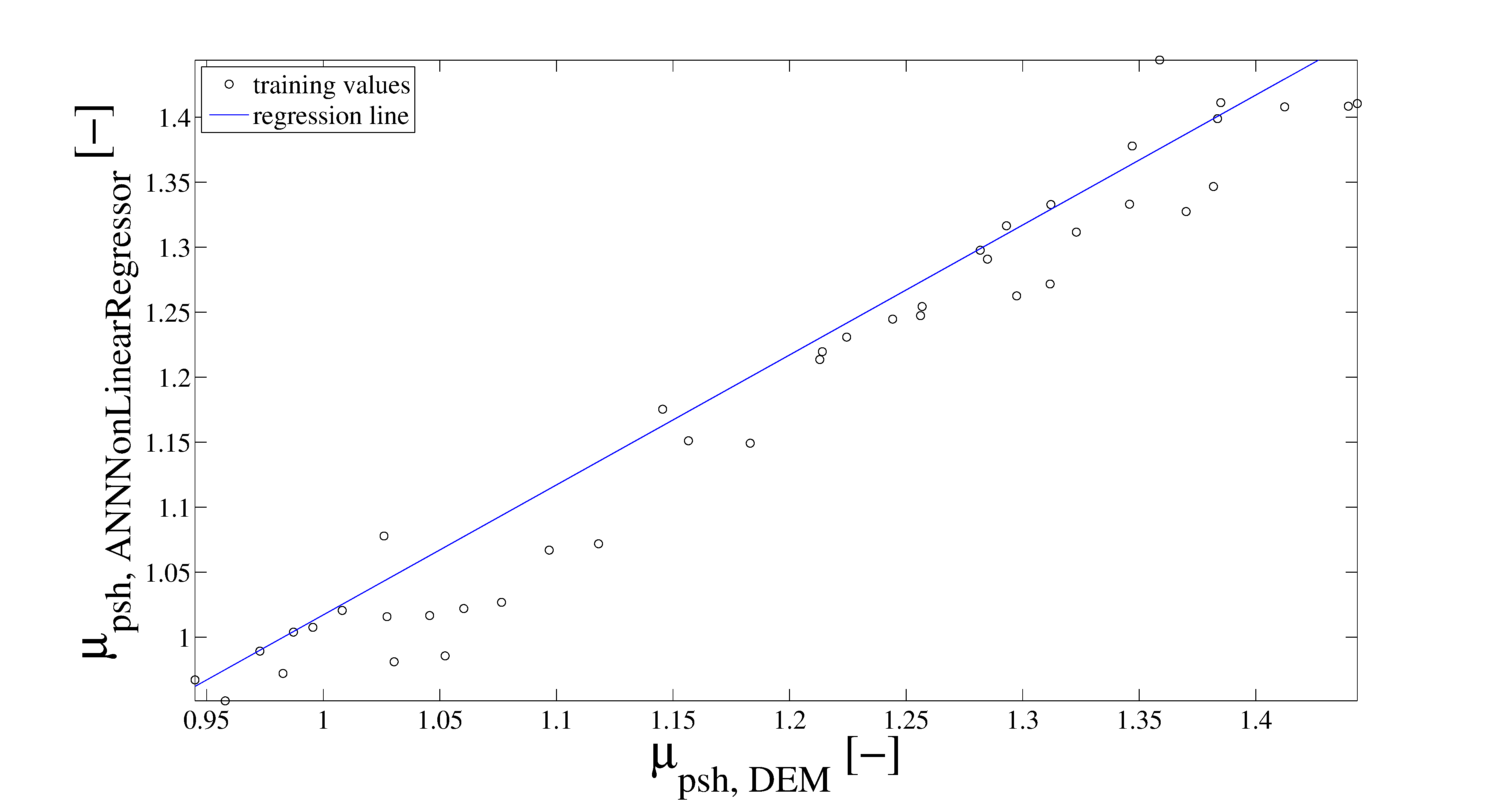
\includegraphics[width=.75\columnwidth]{images/139SCTANNNonLinearRegressor}
	  \label{fig:139SCTANNNonLinearRegressor}
  }
  \caption{Regressions.}
  \label{fig:143sctregressions}
\end{figure}

% \begin{figure}%[!h] 
% \centering 
% 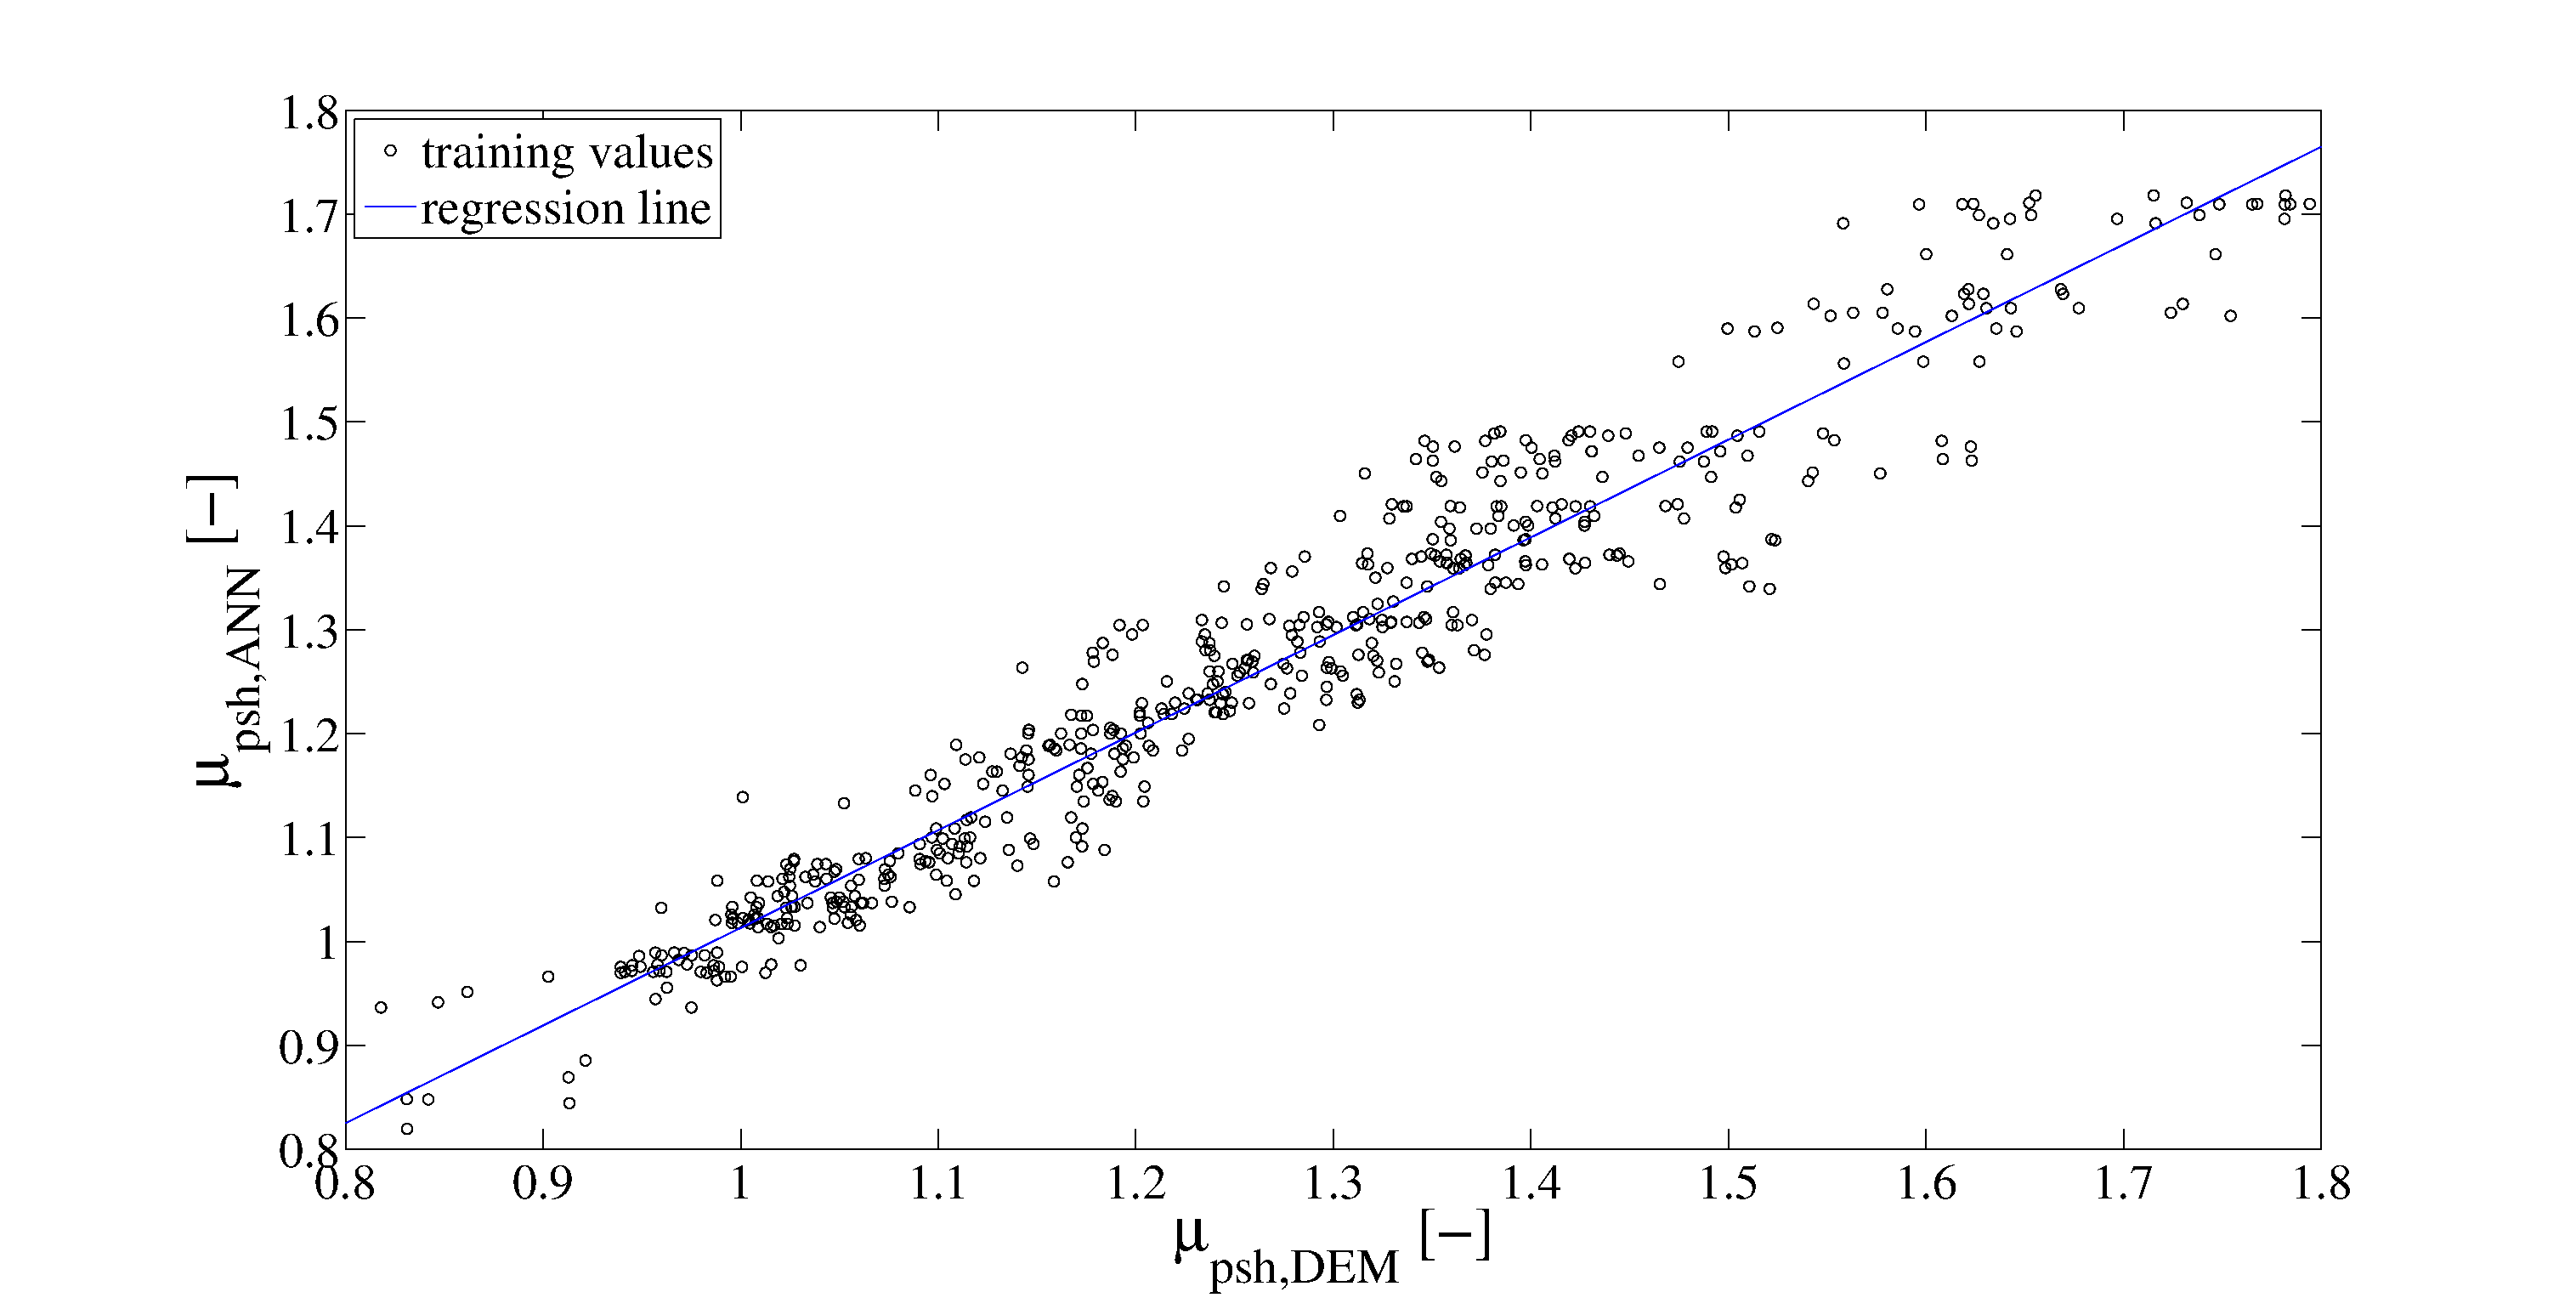
\includegraphics[width=.80\columnwidth]{images/022regression.eps}
% %[width=.48\textwidth]
% \caption[Comparison between prediction of the trained ANN and full DEM
% simulation]{Comparison between prediction of the trained Artificial Neural
% Network (\acs{ANN}) and 546 
% \wrong{write down all the simulations performed at the end.}
% full DEM simulations of the coefficient of pre-shear
% (\acs{mupsh}).}
% \label{fig:022regression} 
% \end{figure}